\chapter{Cálculo modelo de 3 rodas}

\begin{figure}[h]
	\centering
	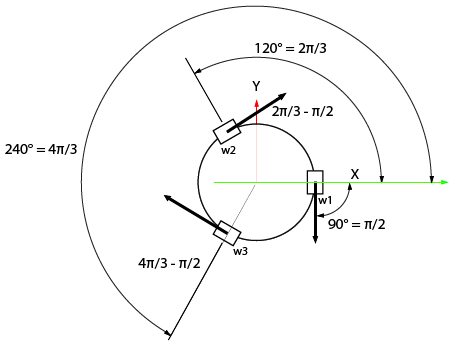
\includegraphics{figures/digram_model_dedution}
	\caption{diagrama do modelo - dedução da matriz}
	\label{lof}
\end{figure}

\begin{equation}
    \begin{split}
        \overrightarrow{V}_{l} = 
        \overrightarrow{V}_{w1}
        + \overrightarrow{V}_{w2}
        + \overrightarrow{V}_{w3}
    \end{split}
\end{equation}

\begin{equation}
    \begin{split}
        \overrightarrow{\omega} = 
        \frac{\vert\overrightarrow{V}_{w1}\vert}{L}
        + \frac{\vert\overrightarrow{V}_{w2}\vert}{L}
        + \frac{\vert\overrightarrow{V}_{w3}\vert}{L}
    \end{split}
\end{equation}


\begin{gather*}
        \dot{V}_{l} \angle \theta =  
        \dot{V}_{w1} \angle \left(-\frac{\pi}{2}\right) 
        + \dot{V}_{w2} \angle \left(\frac{2\pi}{3}-\frac{\pi}{2}\right) 
        + \dot{V}_{w3} \angle \left(\frac{4\pi}{3}-\frac{\pi}{2}\right) 
\end{gather*}

\begin{align*}
    \dot{V}_{l} \cos{ \theta } + j\dot{V}_{l} \sin{\theta} =  
    \dot{V}_{w1} \cos{ \left(-\frac{\pi}{2}\right)} + j\dot{V}_{w1} \sin{ \left(-\frac{\pi}{2}\right) } \\
    + \dot{V}_{w2}  \cos{ \left(\frac{\pi}{6}\right) } + j\dot{V}_{w2}  \sin{ \left(\frac{\pi}{6}\right) }  \\
    + \dot{V}_{w3} \cos{ \left(\frac{5\pi}{6}\right) } + j\dot{V}_{w2}  \sin{ \left(\frac{5\pi}{6}\right) } 
\end{align*}

\begin{equation*}
    \begin{split}
        \dot{\omega} = 
        \frac{\dot{V}_{w1}}{L}
        + \frac{\dot{V}_{w2}}{L}
        + \frac{\dot{V}_{w3}}{L}
    \end{split}
\end{equation*}


\begin{gather}
	\begin{bmatrix} \dot{V}\cdot \cos{\theta} \\  \dot{V}\cdot \sin{\theta} \\  \dot{\omega} \end{bmatrix}
	=
	\begin{bmatrix}
		\cos{\left(-\frac{\pi}{2}\right)} & \cos{\left(\frac{\pi}{6}\right)} & \cos{\left(\frac{5\pi}{6}\right)} \\
		\sin{\left(-\frac{\pi}{2}\right)} & \sin{\left(\frac{\pi}{6}\right)} & \sin{\left(\frac{5\pi}{6}\right)} \\
		\frac{1}{L} & \frac{1}{L} & \frac{1}{L}
	\end{bmatrix}
	\cdot
	\begin{bmatrix} \dot{V}_{w1} \\  \dot{V}_{w2} \\  \dot{V}_{w3} \end{bmatrix}
\end{gather}



\begin{gather}
	\begin{bmatrix} \dot{V}_{w1} \\  \dot{V}_{w2} \\  \dot{V}_{w3} \end{bmatrix}
	=
	\begin{bmatrix}
		0 & 2/3 & L/3 \\
		-1/\sqrt{3} & -1/3 & L/3\\
		1/\sqrt{3} & -1/3 & L/3
	\end{bmatrix}
	\cdot
	\begin{bmatrix} \dot{V}\cdot \cos{\theta} \\  \dot{V}\cdot \sin{\theta} \\  \dot{\omega} \end{bmatrix}
\end{gather}